\documentclass[12pt]{article}

\usepackage{amsmath,amsthm,xspace,multirow}
\usepackage[margin=1in]{geometry}

\usepackage{amsmath} % essential for cases environment
\usepackage{amsthm} % for theorems and proofs
\usepackage{amsfonts} % mathbb
\usepackage{marvosym}
\usepackage{xspace}
\usepackage{multirow} % fancy tables
\usepackage{wasysym} % circle symbols (including half-filled circles)
\usepackage{enumerate} % fancier enumeration (e.g., a,b,c, ...)
%\usepackage{xcolor}
\usepackage{color}
\usepackage{mathtools}
\usepackage{tikz}
\usepackage{oubraces}
\usepackage{hyperref}
\usepackage[toc,page]{appendix}
\usepackage{cleveref}
\usepackage{cite}
\usepackage{textcomp}

\usepackage{algpseudocode,algorithm}
\usepackage{caption}
%used for spacing in list of figures/tables
\usepackage{tocloft}
%predominantly used for list of abbreviations and symbols
\usepackage{longtable}
\usepackage{enumitem}
	\newlist{abbrv}{itemize}{1}
	\setlist[abbrv,1]{label=,labelwidth=1in,align=parleft,itemsep=0.1\baselineskip,leftmargin=!}

%langauge
\usepackage[english]{babel}

%Tabular Commands
\usepackage{array}
\newcolumntype{L}[1]{>{\raggedright\let\newline\\\arraybackslash\hspace{0pt}}m{#1}}
\newcolumntype{C}[1]{>{\centering\let\newline\\\arraybackslash\hspace{0pt}}m{#1}}
\newcolumntype{R}[1]{>{\raggedleft\let\newline\\\arraybackslash\hspace{0pt}}m{#1}}

%make align work with lineno

\newcommand*\patchAmsMathEnvironmentForLineno[1]{%
  \expandafter\let\csname old#1\expandafter\endcsname\csname #1\endcsname
  \expandafter\let\csname oldend#1\expandafter\endcsname\csname end#1\endcsname
  \renewenvironment{#1}%
     {\linenomath\csname old#1\endcsname}%
     {\csname oldend#1\endcsname\endlinenomath}}% 
\newcommand*\patchBothAmsMathEnvironmentsForLineno[1]{%
  \patchAmsMathEnvironmentForLineno{#1}%
  \patchAmsMathEnvironmentForLineno{#1*}}%
\AtBeginDocument{%
\patchBothAmsMathEnvironmentsForLineno{equation}%
\patchBothAmsMathEnvironmentsForLineno{align}%
\patchBothAmsMathEnvironmentsForLineno{flalign}%
\patchBothAmsMathEnvironmentsForLineno{alignat}%
\patchBothAmsMathEnvironmentsForLineno{gather}%
\patchBothAmsMathEnvironmentsForLineno{multline}%
}

%commenting commands
\newcommand{\spenny}[1]{{\color{red}{(\bfseries Spenny: }{\em #1})}}
%\renewcommand{\spenny}[1]{}

%colours

\definecolor{dodgerblue}{RGB}{30,144,255}
\definecolor{darkorchid1}{RGB}{172,29,255}
\definecolor{orange}{RGB}{255,149,0}
\definecolor{forestgreen}{RGB}{0,122,16}
\newcommand{\red}[1]{{\color{red}#1}}

\newtheorem{theorem}{Theorem}[section]
\newtheorem{lemma}{Lemma}[section]
%\renewcommand\qedsymbol{\Coffeecup}
\newcommand{\Note}[1]{\textbf{\emph{Note:}\xspace#1}}
%Greek Letter shortcuts
\newcommand{\lam}{\lambda}
\newcommand{\Lam}{\Lambda}
\newcommand{\gam}{\gamma}
\newcommand{\Gam}{\Gamma}
\newcommand{\eps}{\varepsilon}


\newcommand{\ee}{(\hat{P_1},\hat{P_2},\hat{P_{12}})}
\newcommand{\eep}{\left(1-\frac{\mu}{f_1}\right)}
\newcommand{\eef}{\left(1-\frac{\mu}{f_1},0,0\right)}
\newcommand{\JD}[1]{{\color{blue}{\bfseries Jonathan:} #1}}
\newcommand{\EEZone}{\frac{\beta}{\alpha}\left(1-\frac{\mu}{\gam}\right)}

%Simulation Commands/Macros
\newcommand{\neigh}{{\cal N}}
\newcommand{\state}{\text{state}}
\newcommand{\cmax}[1]{\ensuremath c_{\rm #1}}
\newcommand{\heal}{\text{H}}
\newcommand{\susc}{\text{S}}
\newcommand{\expose}{\text{E}}
\newcommand{\infect}{\text{I}}


%Commenting commands:
\newcommand{\Question}[1]{{\em \bf Question:} #1}
\newcommand{\Answer}[1]{{\em \bf Answer:} #1}

%Unit commands
\newcommand{\mum}{\ensuremath \mu{\rm m}}
\newcommand{\cm}{\ensuremath {\rm cm}}
\newcommand{\mm}{\ensuremath {\rm mm}}

\newcommand{\f}{f}

%Equilibrium macros
\newcommand{\HE}{\textit{HE}\xspace}
\newcommand{\DE}{\textit{DE}\xspace}
\newcommand{\equil}{(\bar{H},\bar{S},\bar{E},\bar{I},\bar{V},\bar{Z})}
\newcommand{\eq}[1]{\overline{#1}}


%% macros
\newcommand{\Reals}{\mathbb{R}}
\newcommand{\term}[1]{{\bfseries\slshape #1}}
\newcommand{\Ker}{{\text{Ker}\,}}
\newcommand{\argmax}{{\text{argmax}}}
\newcommand{\argmin}{{\text{argmin}}}
\newcommand{\Range}{{\text{Range}\,}}
\newcommand{\norm}[1]{\left\|#1\right\|}
\newcommand{\abs}[1]{\left|#1\right|}
\newcommand{\R}{{\cal R}}
\newcommand{\G}{{\cal G}}
\newcommand{\N}{{\cal N}}
\newcommand{\Tinf}{T_\textrm{inf}}
\newcommand{\Prob}{\textrm{Pr}}
\newcommand{\Shat}{{\hat{S}}}
\newcommand{\Ihat}{{\hat{I}}}
\newcommand{\ie}{\emph{i.e., }}
\newcommand{\eg}{\emph{e.g., }}
% \newcommand{\Rlogo}{\protect\includegraphics[height=2ex,keepaspectratio]{images/Rlogo.pdf}\xspace}
\newcommand{\Rlogo}{\textbf{\textsf{R}}\xspace}
\newcommand{\XPPAUT}{\texttt{XPPAUT}\xspace}
\newcommand{\etal}{\textit{et al}.\xspace}
\newcommand\emphblue[1]{\emph{\color{blue}#1}}
\newcommand{\citehere}{{\large \bf CITE HERE}}

%derivative notation
\newcommand{\D}[2]{\frac{\mathrm{d}#1}{\mathrm{d}#2}}
\newcommand{\partD}[2]{\frac{\partial \mathrm{d}#1}{\partial #2 			\mathrm{d}t}}
\newcommand{\at}[2][]{\left. #1\right|_{#2}}
\newcommand{\partd}[2]{\frac{\partial #1}{\partial #2}}
\newcommand{\x}{\text{\bf x}}
\newcommand{\Mod}[1]{\ (\text{mod}\ #1)}
%THESE ARE SPENCER'S MACROSSSSSSS

\newcommand{\A}{\frac{\alpha\delta(\rho+\chi)}{\chi\beta f}}
\newcommand{\perday}{{$\text{day}^{-1}$\xspace}}

%Text Macros
\newcommand{\TM}{\textsuperscript{TM}\xspace}

\definecolor{dkgreen}{rgb}{0,0.6,0}
\definecolor{gray}{rgb}{0.5,0.5,0.5}
\definecolor{mauve}{rgb}{0.58,0,0.82}

%-----------------
% Listings Package for code script
%-----------------
\usepackage{listings}


\lstset{ %
  language=R,                     % the language of the code
  basicstyle=\footnotesize\ttfamily,       % the size of the fonts that are used for the code
  numbers=left,                   % where to put the line-numbers
  numberstyle=\tiny\color{gray},  % the style that is used for the line-numbers
  stepnumber=1,                   % the step between two line-numbers. If it's 1, each line
                                  % will be numbered
  numbersep=5pt,                  % how far the line-numbers are from the code
  backgroundcolor=\color{white},  % choose the background color. You must add \usepackage{color}
  showspaces=false,               % show spaces adding particular underscores
  showstringspaces=false,         % underline spaces within strings
  showtabs=false,                 % show tabs within strings adding particular underscores
  frame=none,                   % adds a frame around the code
  rulecolor=\color{black},        % if not set, the frame-color may be changed on line-breaks within not-black text (e.g. commens (green here))
  tabsize=2,                      % sets default tabsize to 2 spaces
  captionpos=b,                   % sets the caption-position to bottom
  breaklines=true,                % sets automatic line breaking
  breakatwhitespace=false,        % sets if automatic breaks should only happen at whitespace
  title=\lstname,                 % show the filename of files included with \lstinputlisting;
                                  % also try caption instead of title
  keywordstyle=\color{blue},      % keyword style
  commentstyle=\color{dkgreen},   % comment style
  stringstyle=\color{mauve},      % string literal style
  escapeinside={\%*}{*)},         % if you want to add a comment within your code
  morekeywords={*,...}            % if you want to add more keywords to the set
} 



\usepackage{tikz}
\usetikzlibrary{
arrows,decorations.pathmorphing,backgrounds,positioning,fit,calc,scopes,shapes.misc
}


\tikzset{
	auto,
	compartment/.style={
		rectangle, minimum size=9mm, rounded corners=2mm,
		thick, draw=black!15, top color=white,bottom color=black!30
	},
	%
	bigcompartment/.style={
		rectangle, minimum size=24mm, rounded corners=5mm,
		thick, draw=black!15, top color=white,bottom color=black!20
	},
	%
	point/.style={
		circle, inner sep=2pt, fill=black!5
	},
	%
	mytextbox/.style={
		rectangle, text=black!50, thin, 
		draw=white, top color=white,bottom color=white, fill=white
	}
	
}

\tikzset{cross/.style={cross out, draw=black, minimum size=2*(#1-\pgflinewidth), inner sep=0pt, outer sep=0pt},
%default radius will be 1pt. 
cross/.default={5pt}}

\newcommand{\SIRboxes}
{
\node (S) [bigcompartment,bottom color=blue!30]{{S}};
\node (SI) [right=of S]{};
\node (I) [bigcompartment,right=of SI,bottom color=red!30]{I};
\node (IR) [right=of I]{};
\node (R) [bigcompartment,right=of IR,bottom color=green!30]{R};
}
\newcommand{\sirvec}[2]{ 
	\draw[->, very thick] (S) to node[midway]{#1}(I) ;
	%\node (SIparam) [above of= SI]{#1}; 
	\draw[->, very thick] (I) to node[midway]{#2}(R);
	%\node (IRparam) [above of=IR]{#2}; 
}


\newcommand{\sirs}[1]{ 
	\draw[->, very thick] (R) 
		to  [bend left=45] node[midway] {#1} (S) ;
		 
}


\newcommand{\SIboxes}
{
\node (S) [bigcompartment,bottom color=blue!30]{{S}};
\node (SI) [right=of S]{};
\node (I) [bigcompartment,right=of SI,bottom color=red!30]{I};
}

\newcommand{\sivec}[1]{ 
	\draw[->, very thick] (S) to node[midway]{#1}(I) ;
	%\node (SIparam) [above of= SI]{#1};  
}

\newcommand{\sis}[1]
{
	\draw[->, very thick] (I) 
		to  [bend left=45] node[midway] {#1} (S) ;
}

\newcommand{\SILboxes}
{
\node (S) [bigcompartment,bottom color=blue!30]{S};
\node (SI) [right= of S]{};
\node (I) [bigcompartment,right=of SI,bottom color=red!30]{I};
\node (IL) [right=of I]{};
\node (L) [bigcompartment,right=of IL,bottom color=yellow!30]{L};
}







%\newcommand{\D}[2]{\frac{\mathrm{d}#1}{\mathrm{d}#2}}
%\newcommand{\ie}{\emph{i.e., }}
%\newcommand{\eg}{\emph{e.g., }}

\usepackage{tikz}
\newdimen\mylw
\tikzset{chemeq/.style={draw,thick,double distance=2pt,onearc-onearc,/chemeq/size={#1}}}
\tikzset{chemeq/.default={.4pt 6pt}}
\pgfkeys{/chemeq/size/.code={\pgfsetarrowoptions{onearc}{#1}}}
\def\parseopts#1 #2{\xdef\myalw{#1}\xdef\myasize{#2}}
\pgfarrowsdeclare{onearc}{onearc}{%
  {\edef\x{\pgfgetarrowoptions{onearc}}\expandafter\parseopts\x}
  \mylw=\myalw
  \pgfarrowsleftextend{-\myasize-.5\mylw}
  \pgfarrowsrightextend{0pt}
}{%
  \pgfsetdash{}{0pt}
  {\edef\x{\pgfgetarrowoptions{onearc}}\expandafter\parseopts\x}
  \mylw=\pgflinewidth
  \pgfsetlinewidth{\myalw}
  \pgfpathmoveto{\pgfpoint{-\myasize}{-\myasize-.5\mylw}}%
  \pgfpatharc{180}{90}{\myasize}
  \pgfusepathqstroke
}

\title{HPV Vaccination of Boys and Men}

\begin{document}
\maketitle

\section{Introduction}

The human papillomavirus (HPV) is a virus which infects epithelial and mucosal cells.  There are over 100 different types of HPV, over 40 of which are sexually transmitted.  HPV types are categorized as high-risk or low-risk based on their association with various cancers.  HPV-16 and HPV-18 are two of the most oncogenic HPV types and are associated with a number of cancers in the anogenital and oropharyngeal tracts.  To combat the burden of these two HPV types, two vaccines have been developed to protect against these two types.  Cervarix is a bivalent vaccine (HPV2) manufactured by GlaxoSmithKlein.  Gardasil is a quadravalent vaccine (HPV4), and in addition to protecting against HPV-16 and -18, it also protects against HPV-6 and -11, two HPV types highly associated with genital warts.  While these vaccines are relatively young, studies show that these vaccines have high efficacy in protecting against these specific HPV types and are believed to relieve the burden of cervical cancer and other associated cancers.  

According to the Canada Communicable Disease Report developed by the Public Health Agency of Canada, Health Canada has authorized the use of HPV4 and HPV2 in female populations aged 9-26 years to protect against cancers associated with HPV-16 and -18.  HPV4 has reported protective effects against vaginal, vulvar, and cervical cancers and precursors up to age 45 in women.  Only HPV4 (Gardasil) approved for use in males (9-26 years) to protect against infections of HPV types 6, 11, 16, and 18.  Furthermore, vaccination recommendations from PHAC include vaccinating females aged 9-13 years  with either vaccine to protect against these HPV types before the onset of sexual activity.  The PHAC also recommends vaccinating males with HPV4 between the ages of 9 and 26 years to prevent associated anal and penile diseases.  PHAC also makes a specific recommendation to vaccinate MSM greater than 9 years of age.  

While the PHAC has recommended vaccinating men with HPV4 to protect against diseases associated with HPV types 6, 11, 16, and 18, only few provinces have included boys in their routine vaccination programme.  Currently, only three provinces administer the HPV vaccine routinely to both boys and girls.  In 2016, Manitoba will include boys in their routine HPV vaccination schedule of grade 6 students, with a catch-up vaccination of boys in grade 9.  Some provinces provide vaccination of boys with HIV such as Quebec and British Columbia.  As of September 2015, British Columbia include at risk males in their vaccination programme.  This includes boys who identify as MSM or questioning, boys who are street-involved, or those who have HIV. While this particular program targets at risk boys, vaccine uptake will be based on self-reported identification within these groups, and thus could result in significant under vaccination.  Moreover, many boys who may identify as MSM or questioning their sexuality may not realize at this age and could miss the vaccine entirely.  See Table~\ref{tab:ImmuneSched} for the entire list of HPV vaccination procedures for each province and territory.  

Studies have shown that the HPV4 vaccine has significant and efficacious protective effects against HPV infection and related diseases in men.  Despite federal, provincial, and territorial government health organizations recommending boys be vaccinated with HPV4, only three provinces currently include all boys in their routine immunization schedule (4 provinces starting in September 2016).  While British Columbia is included at-risk boys in their routine schedule, the potential for low vaccine uptake is high, given that many boys are not comfortable disclosing information of this kind at that age, or could even be unaware at that point in their sexual development.  

We develop a simple transmission model for HPV, including both boys and girls in the transmission mechanism.  We also consider a queer perspective in this model by including same-sex transmission of HPV.  To disentangle the specific effects of HPV transmission of MSM, we have separated the males into exclusive heterosexual (denoted $h$) and queer (denoted $q$).  We consider a variety of vaccination strategies with variable vaccine efficacy to examine these effects on HPV prevalence.  
\section*{Previous Work - Marek's Work}

Marek Smieja and a small research group began examining this problem during a workshop.  They set up a simple HPV transmission model in men and women.  They consider three infection status groups for both men and women: susceptible, infected, and vaccinated.  Individuals enter the model when they become sexually active (they assume age 15) at a rate $b_iN_i$, where $b_i$ is the birthrate for gender $i$ and $N_i$ is the number of individuals of gender $i$.  Individuals are separated into vaccinated or susceptible at a particular vaccination rate $v_i$ for gender $i$.  

Transmission is considered based on sexual interactions between men and women.  They consider same-sex interactions in men and women, but due to the lack of same-sex data, they set these parameters to zero when fitting the data.  The transmission of HPV in women is expressed as follows (analogously for men):
\begin{equation}
S_{W}\left(\beta_{fm}\frac{I_M}{N_M} + \beta_{ff}\frac{I_W}{N_W}\right)
\end{equation}
where $\beta_{fm}$ and $\beta_{ff}$ is the transmission of HPV onto women from men and women, respectively.  When an individuals is infected, they can clear the infection at a rate $\gamma_i$ after which the individual becomes susceptible again.  There is evidence that natural infections do not provide much protection from subsequent re-infection and does not protect significantly from infections of other HPV types.  

They also consider the vaccination isn't 100\% effective or long lasting. Vaccinated individuals' protection wanes at a rate of $w_i$ for gender $i$, after which they become fully susceptible.  Vaccinated individuals also have a protective factor of $\eps\in[0,1]$, which scales HPV transmission.  That is $\eps=0$ is full protection and $\eps=1$ is no protection.  

We adapt this model by separating the male group into two different subgroups: straight males $M$ and men who have sex with men (queer men) $Q$. In this way we can examine the effects of vaccination strategies on men and queer men.  There is a concern that the female-only vaccination strategies provide little to no herd immunity to MSM and thus they may become a reservoir for HPV. 

\section*{Adaptations to the Model}

As previously mentioned we separate the men into straight men $M$ and queer men $Q$.  Queer men have sexual interactions with both men and and women.  The proportion of same-sex interactions in men is $p$ and the proportion of same-sex interactions in women is $q$.  In this way we set up three different HPV transmission terms:

We examine the transmission of HPV in straight males.  These individuals can be infected by women solely.  
\begin{equation}
S_M\left(\frac{(1-q)\beta_{mf}I_W}{N_W}\right)
\end{equation}
Queer men can be infected by both other MSM and also women.
\begin{equation}
S_Q\left(\frac{p^2\beta_{mm}I_Q}{N_Q}+\frac{(1-p)(1-q)\beta_{mf}I_W}{N_W}\right)
\end{equation}
Women can be infected by both straight and queer men, and we also consider same sex interactions in women. 
\begin{equation}
S_W\left(\frac{(1-q)\beta_{fm}I_M}{N_M}+\frac{(1-q)(1-p)\beta_{fm}I_Q}{N_Q}+\frac{q^2\beta_{ff}I_W}{N_W}\right)
\end{equation}
We set up the entire model as a flow diagram.  The flow diagram for straight men is illustrated in Figure~\ref{fig:flowMen} and in MSM in Figure~\ref{fig:flowQueer}.  
\begin{figure}[h!]
\begin{center}
\resizebox{0.7\textwidth}{!}{
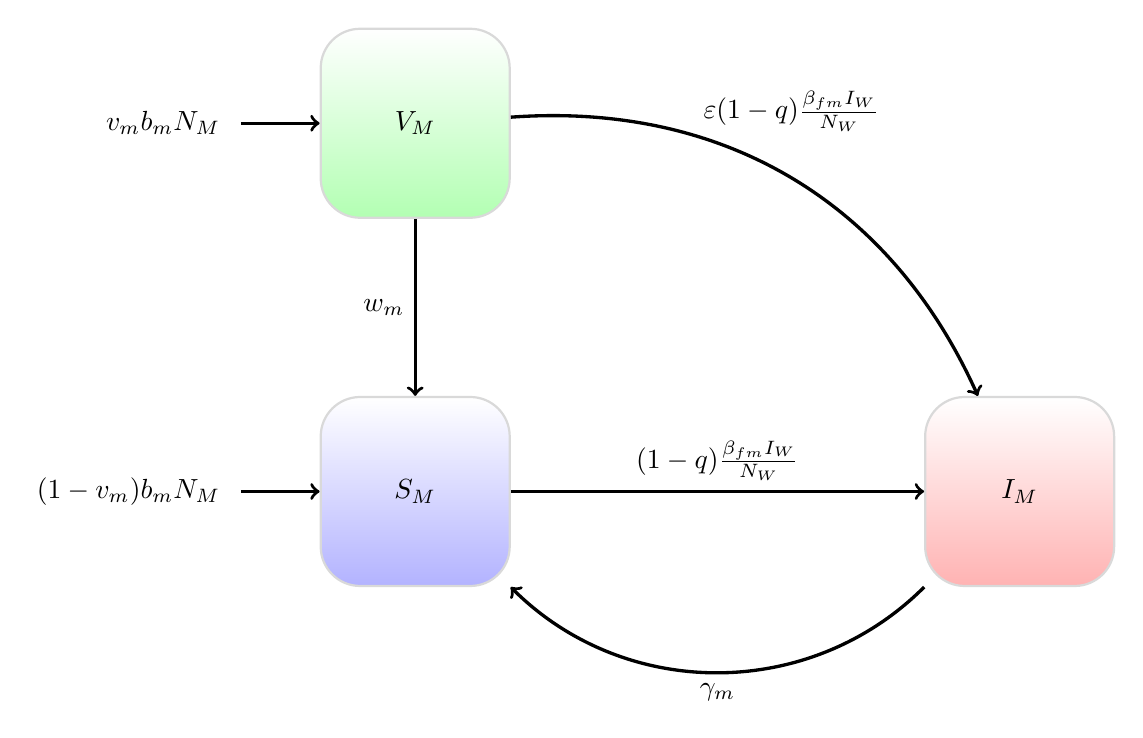
\begin{tikzpicture}
%compartments
\node (SM)[bigcompartment, bottom color=blue!30] {{$S_M$}};
\node (SIM) [right=of SM,xshift=3cm]{{}};
\node (SVM) [above=of SM]{};

\node (IM) [bigcompartment,right=of SIM,bottom color=red!30]{{$I_M$}};
\node (VM) [bigcompartment,above=of SVM,bottom color=green!30]{{$V_M$}};
\node (leftSM) [left=of SM]{{}};
\node (leftVM) [left=of VM]{};

%arrows
\draw[very thick, ->] (leftSM) node[left]{$(1-v_m)b_mN_M$} to  (SM);
\draw[very thick, ->] (leftVM) node[left]{$v_mb_mN_M$} to  (VM);

\draw[very thick,->] (VM) to node[left]{$w_m$} (SM);

\draw[very thick,->] (SM) to node[above]{$(1-q)\frac{\beta_{fm}I_W}{N_W}$} (IM);
\draw[very thick,->] (VM) to[bend left=35] node[above,yshift=3ex]{$\eps(1-q)\frac{\beta_{fm}I_W}{N_W}$} (IM);
\draw[very thick,->] (IM) to[bend left=45] node[below] {$\gamma_m$} (SM);
\end{tikzpicture}
}% end resize box
\end{center}
\caption{HPV Transmission flow diagram for straight men.}
\label{fig:flowMen}
\end{figure}
%
\begin{figure}[h!]
\begin{center}
\resizebox{0.7\textwidth}{!}{
\begin{tikzpicture}
%compartments
\node (S)[bigcompartment, bottom color=blue!30] {{$S_Q$}};
\node (SI) [right=of S,xshift=3cm]{{}};
\node (SV) [above=of S]{};

\node (I) [bigcompartment,right=of SIM,bottom color=red!30]{{$I_Q$}};
\node (V) [bigcompartment,above=of SVM,bottom color=green!30]{{$V_Q$}};
\node (leftSQ) [left=of S]{{}};
\node (leftVQ) [left=of V]{};

%arrows
\draw[very thick, ->] (leftSQ) node[left]{$(1-v_m)b_mN_Q$} to  (S);
\draw[very thick, ->] (leftVQ) node[left]{$v_mb_mN_Q$} to  (V);

\draw[very thick,->] (V) to node[left]{$w_m$} (S);

\draw[very thick,->] (S) to node[above]{$\frac{p^2\beta_{mm}I_Q}{N_Q}+\frac{(1-p)(1-q)\beta_{mf}I_W}{N_W}$} (I);
\draw[very thick,->] (V) to[bend left=35] node[above,yshift=3ex]{$\eps(\frac{p^2\beta_{mm}I_Q}{N_Q}+\frac{(1-p)(1-q)\beta_{mf}I_W}{N_W})$} (I);
\draw[very thick,->] (I) to[bend left=45] node[below] {$\gamma_m$} (S);
\end{tikzpicture}
}% end resize box
\end{center}
\caption{HPV Transmission flow diagram for men who have sex with men.}
\label{fig:flowQueer}
\end{figure}
The diagram for women is similar to these with the appropriate transmission terms and parameters outlined above. This translates to a system of differential equations:
\begin{align}
\D{S_i}{t}&=(1-v_i)d_iN_i + w_iV_I - \lambda_iS_i + \gamma_iI_i - d_iS_i,\\
\D{I_i}{t}&= \lambda_iS_i - \gamma_iI_i- d_iI_i,\\
\D{V_i}{t}&= v_id_iN_i - w_iV_i - \eps \lambda_iV_i - d_iV_i.
\end{align}
where $i$ refers to either straight men, queer men, or women.  The parameter $\lambda_i$ is the force of transmission and is a function of mixing rates.  

\subsection*{Sexual Mixing}

In our model, we consider both straight and queer individuals.  Because women are vaccinated against HPV in the current immunization program, we combine straight women and queer women in the same group, referred to as women.  Because men are not included in the immunization program, and because queer men may not benefit from women-vaccinated herd immunity, we keep these two groups separate, denoted as heterosexual men and queer men.  Queer men have sex with both men and women, while heterosexual men have sex with solely women.  

We set up a mixing rate of an individual in group $i$ with those in group $j$ as $m_{ij}$.  Mixing here must be symmetrical; that is $m_{ij}=m_{ji}$.  The mixing rate is calculated as such
\begin{equation}
m_{ij} = c_i n_i p_{ij}
\end{equation}
where $c_i$ is the average contact rate of group $i$, $n_i$ is the relative number of individuals in group $i$, and $p_{ij}$ is the probability of and individual in group $i$ mixing with someone from group $j$.  Because mixing is symmetric, we have the following constraint
\begin{equation}
m_{ij} = c_i n_i p_{ij} = c_j n_j p_{ji} = m_{ji}
\end{equation}
We also have the following constraint in that the sum of the mixing probabilities over all groups $j$ must equal 1. 
\begin{equation}
\sum_j p_{ij} = 1
\end{equation}
To simplify solving the this system, we set $r_{ij}=c_ip_{ij}$ and choose values of $r_{ij}$ that work based on given values of $n_i$.  Then from the previous constraint we have:
\begin{equation}\label{eq:ContRateEq}
\sum_j r_{ij} = c_i \sum_j p_{ij} = c_i
\end{equation}
And thus we have that 
\begin{equation}\label{eq:ProbEq}
p_{ij}=\frac{r_{ij}}{c_i}
\end{equation}

\subsection*{Dummy Value Example}

The following is a dummy example calculation.  I consider the proportional number of individuals.  That is that $n_w=n_m=0.5$ where the number of men $n_m=n_h+n_q$ is the sum of all heterosexual and queer men.  Under the assumption that about 20\% of men are queer, we solve for $n_h$ and $n_q$ accordingly
\begin{align}
n_h&=0.8n_m = 0.8(0.5) = 0.4\\
n_q&=0.2n_m = 0.2(0.5) = 0.1
\end{align}
Because we know that $m_{ij}=m_{ji}$ so we can solve for some values of $r_{ij}$ by choosing other values.  Based on the structure of our model, we separate men into heterosexual exclusive and queer men.  Thus heterosexual men only sexually interact with women, and not other heterosexual men or queer men. Thus, $r_{hh}=r_{hq}=r_{qh}=0$.  We also start setting some $r_{ij}$ values and solving for others that maintain $m_{ij}=m_{ji}$, that is
\begin{equation}
r_{ji}=\frac{n_ir_{ij}}{n_j}
\end{equation}
So I chose $r_{hw}=3$, $r_{qq}=5$, and $r_{qw}=1$, and $r_{ww}=0.25$.  Then I solved for the $R$ matrix
\begin{equation}
R=\left(\begin{array}{c c c}
0 & 0 & 3 \\
0 & 5 & 1 \\
2.4 & 0.2 & 0.25
\end{array}\right)
\end{equation}
which gives a mixing matrix of 
\begin{equation}
M=\left(\begin{array}{c c c}
0 & 0 & 1.2 \\
0 & 0.5 & 0.1 \\
1.2 & 0.1 & 0.125
\end{array}\right)
\end{equation}
We can then solve for the contact rates for each group using Equation \eqref{eq:ContRateEq}, which gives $c_h=3$, $c_q=6$, and $c_w=2.85$. And we can use Equation \eqref{eq:ProbEq} and we obtain the matrix $P$ which gives the probability of interaction of someone from group $i$ mixing with someone in group $j$. 
\begin{equation}
P=\left(\begin{array}{c c c}
0 & 0 & 1 \\
0 & 0.833 & 0.167 \\
0.842 & 0.070 & 0.088
\end{array}\right)
\end{equation}

\spenny{I don't really know if this is what you had in mind.  We would most likely calculate this from data, so I would like to see how this model translates to data and then try to figure out how to calculate it back.  That is what I would like to discuss.  }
\section*{Parameter Values}

I have taken the parameter values from the model that Marek et al. used in their project, and adapted them slightly. They set the parameter $\gamma$ based on prior knowledge about HPV clearance times, and fit the model to data to estimate $\beta$. They let vaccination parameters $v$, $w$, and $\eps$ be variable parameters in the model to examine the effects of various vaccination strategies on the prevalence of HPV in the population.

Most HPV infections are fully cleared after an average of 16 months.  Thus they set $\gamma=1/16$ month\textsuperscript{-1}.  By fitting the model to population level data in Ontario they estimate a $\beta=0.0845$ month\textsuperscript{-1}.  They don't differentiate between male-to-female or female-to-male transmission, so I assume that this is male-to-female transmission, and thus $\beta_{fm}=0.0845$ in the dummy model.  Because we consider various sexual mixing scenarios, I altered the transmission rates based on prior knowledge about HPV disease dynamics.  It has been shown that female-to-male HPV transmission is less common (apart from oropharyngeal HPV) thus I set $\beta_{mf}=0.0800$ month\textsuperscript{-1}.  Furthermore, female-to-female transmission is thought to be even less common, so I set $\beta_{ff}=0.0700$.  It is also thought that male-to-male transmission is greater than that of $\beta_{fm}$ so I set this value to be $\beta_{mm}=0.0900$ month\textsuperscript{-1}.  Because these values are anecdotal guesses, not much weight should be put into the accuracy of these values.  They purely provide a means by which to develop a skeletal model for fitting at a later date. 

In terms of sexual mixing, I have also anecdotally guess the proportion of same-sex interactions for women and queer men. 


\section*{Additional Information}
\begin{table}[h!]
\begin{center}
\begin{tabular}{l | l | l }
Province/Territory & Routine &  As of (year)\\
\hline
\hline
\multirow{2}{*}{British Columbia} & Grade 6 girls & \multirow{2}{*}{2015}\\
& At Risk Boys\textsuperscript{*} & \\
\hline
Alberta & Grade 5 girls and boys & 2014\\
\hline
Saskatchewan & Grade 6 girls & 2015\\
\hline
\multirow{2}{*}{Manitoba} & Grade 6 girls & 2015\\
& Grade 6 girls and boys & Starting 2016\\
\hline 
Ontario & Grade 8 girls & 2015\\
\hline
Qu\'{e}bec & Grade 4 girls & 2015\\
\hline 
New Brunswick & Grade 7 girls & 2015 \\
\hline 
Nova Scotia & Grade 7 girls and boys & 2015\\
\hline
Prince Edward Island & Grade 8 girls and boys & 2015\\
\hline
NFLD and Labrador & Grade 6 girls & 2015\\
\hline
Yukon & Grade 6 girls & 2014\\
\hline
Northwest Territories & Grade 4-6 girls & 2015\\
\hline 
Nunavut & Grade 6 girls & NA\\
\hline
\end{tabular}

\caption{Current immunization schedule by province and territory for HPV.  Gathered from provincial and territorial health websites.  \newline
{\footnotesize \textsuperscript{*} At risk boys includes MSM or those questioning their sexuality, street-involved, or HIV-infected}}
\label{tab:ImmuneSched}
\end{center}
\end{table}

\end{document}
\newpage
\bibliographystyle{plain}
\bibliography{NotesBib}

\end{document}